% FreqODES -- 22AIE437 Medical Image Processing final project presentation
% Compile: pdflatex main (run twice; no BibTeX pass needed) -- or upload to Overleaf
\documentclass[aspectratio=169,10pt]{beamer}
\usetheme{Madrid}
\usecolortheme{beaver}
\setbeamertemplate{navigation symbols}{}
\setbeamertemplate{caption}[numbered]
\usepackage[utf8]{inputenc}
\usepackage{booktabs,multirow,graphicx,amsmath,xcolor}
\usepackage{tikz}
\usetikzlibrary{arrows.meta,positioning,shapes.geometric,fit,backgrounds}

\newcommand{\DBNKTennoDW}{78.48}
\newcommand{\JBNKTennoDW}{--}
\newcommand{\TBNKTennoDW}{176}
\newcommand{\DBNKTennoDWLiver}{87.71}
\newcommand{\JBNKTennoDWLiver}{--}
\newcommand{\DBNKTennoDWLK}{75.86}
\newcommand{\JBNKTennoDWLK}{--}
\newcommand{\DBNKTennoDWRK}{73.33}
\newcommand{\JBNKTennoDWRK}{--}
\newcommand{\DBNKTennoDWSpleen}{77.01}
\newcommand{\JBNKTennoDWSpleen}{--}
\newcommand{\DBNKTen}{78.38}
\newcommand{\JBNKTen}{--}
\newcommand{\TBNKTen}{176}
\newcommand{\DBNKTenLiver}{87.70}
\newcommand{\JBNKTenLiver}{--}
\newcommand{\DBNKTenLK}{75.59}
\newcommand{\JBNKTenLK}{--}
\newcommand{\DBNKTenRK}{73.51}
\newcommand{\JBNKTenRK}{--}
\newcommand{\DBNKTenSpleen}{76.71}
\newcommand{\JBNKTenSpleen}{--}
\newcommand{\DBNKFifty}{79.26}
\newcommand{\JBNKFifty}{--}
\newcommand{\TBNKFifty}{181}
\newcommand{\DBNKFiftyLiver}{87.82}
\newcommand{\JBNKFiftyLiver}{--}
\newcommand{\DBNKFiftyLK}{76.99}
\newcommand{\JBNKFiftyLK}{--}
\newcommand{\DBNKFiftyRK}{74.71}
\newcommand{\JBNKFiftyRK}{--}
\newcommand{\DBNKFiftySpleen}{77.51}
\newcommand{\JBNKFiftySpleen}{--}
\newcommand{\DDWTKTen}{77.33}
\newcommand{\JDWTKTen}{--}
\newcommand{\TDWTKTen}{116}
\newcommand{\DDWTKTenLiver}{86.92}
\newcommand{\JDWTKTenLiver}{--}
\newcommand{\DDWTKTenLK}{74.47}
\newcommand{\JDWTKTenLK}{--}
\newcommand{\DDWTKTenRK}{71.95}
\newcommand{\JDWTKTenRK}{--}
\newcommand{\DDWTKTenSpleen}{75.99}
\newcommand{\JDWTKTenSpleen}{--}
\newcommand{\DDWTKFifty}{78.97}
\newcommand{\JDWTKFifty}{--}
\newcommand{\TDWTKFifty}{120}
\newcommand{\DDWTKFiftyLiver}{87.69}
\newcommand{\JDWTKFiftyLiver}{--}
\newcommand{\DDWTKFiftyLK}{76.68}
\newcommand{\JDWTKFiftyLK}{--}
\newcommand{\DDWTKFiftyRK}{74.16}
\newcommand{\JDWTKFiftyRK}{--}
\newcommand{\DDWTKFiftySpleen}{77.34}
\newcommand{\JDWTKFiftySpleen}{--}
\newcommand{\DFFTKTen}{77.31}
\newcommand{\JFFTKTen}{--}
\newcommand{\TFFTKTen}{116}
\newcommand{\DFFTKTenLiver}{86.69}
\newcommand{\JFFTKTenLiver}{--}
\newcommand{\DFFTKTenLK}{73.43}
\newcommand{\JFFTKTenLK}{--}
\newcommand{\DFFTKTenRK}{72.21}
\newcommand{\JFFTKTenRK}{--}
\newcommand{\DFFTKTenSpleen}{76.93}
\newcommand{\JFFTKTenSpleen}{--}
\newcommand{\DFFTKFifty}{79.34}
\newcommand{\JFFTKFifty}{--}
\newcommand{\TFFTKFifty}{123}
\newcommand{\DFFTKFiftyLiver}{87.89}
\newcommand{\JFFTKFiftyLiver}{--}
\newcommand{\DFFTKFiftyLK}{77.39}
\newcommand{\JFFTKFiftyLK}{--}
\newcommand{\DFFTKFiftyRK}{74.63}
\newcommand{\JFFTKFiftyRK}{--}
\newcommand{\DFFTKFiftySpleen}{77.43}
\newcommand{\JFFTKFiftySpleen}{--}
\newcommand{\DFREQKTennoDW}{77.30}
\newcommand{\JFREQKTennoDW}{--}
\newcommand{\TFREQKTennoDW}{116}
\newcommand{\DFREQKTennoDWLiver}{86.71}
\newcommand{\JFREQKTennoDWLiver}{--}
\newcommand{\DFREQKTennoDWLK}{74.45}
\newcommand{\JFREQKTennoDWLK}{--}
\newcommand{\DFREQKTennoDWRK}{72.19}
\newcommand{\JFREQKTennoDWRK}{--}
\newcommand{\DFREQKTennoDWSpleen}{75.86}
\newcommand{\JFREQKTennoDWSpleen}{--}
\newcommand{\DFREQKTen}{77.65}
\newcommand{\JFREQKTen}{--}
\newcommand{\TFREQKTen}{117}
\newcommand{\DFREQKTenLiver}{86.79}
\newcommand{\JFREQKTenLiver}{--}
\newcommand{\DFREQKTenLK}{74.53}
\newcommand{\JFREQKTenLK}{--}
\newcommand{\DFREQKTenRK}{72.26}
\newcommand{\JFREQKTenRK}{--}
\newcommand{\DFREQKTenSpleen}{77.03}
\newcommand{\JFREQKTenSpleen}{--}
\newcommand{\DFREQKFifty}{78.91}
\newcommand{\JFREQKFifty}{--}
\newcommand{\TFREQKFifty}{123}
\newcommand{\DFREQKFiftyLiver}{87.76}
\newcommand{\JFREQKFiftyLiver}{--}
\newcommand{\DFREQKFiftyLK}{76.67}
\newcommand{\JFREQKFiftyLK}{--}
\newcommand{\DFREQKFiftyRK}{73.96}
\newcommand{\JFREQKFiftyRK}{--}
\newcommand{\DFREQKFiftySpleen}{77.24}
\newcommand{\JFREQKFiftySpleen}{--}
\newcommand{\DFUSEDKTenLQuarter}{78.11}
\newcommand{\JFUSEDKTenLQuarter}{--}
\newcommand{\TFUSEDKTenLQuarter}{178}
\newcommand{\DFUSEDKTenLQuarterLiver}{87.24}
\newcommand{\JFUSEDKTenLQuarterLiver}{--}
\newcommand{\DFUSEDKTenLQuarterLK}{75.29}
\newcommand{\JFUSEDKTenLQuarterLK}{--}
\newcommand{\DFUSEDKTenLQuarterRK}{73.34}
\newcommand{\JFUSEDKTenLQuarterRK}{--}
\newcommand{\DFUSEDKTenLQuarterSpleen}{76.56}
\newcommand{\JFUSEDKTenLQuarterSpleen}{--}
\newcommand{\DFUSEDKTenLFifty}{78.15}
\newcommand{\JFUSEDKTenLFifty}{--}
\newcommand{\TFUSEDKTenLFifty}{178}
\newcommand{\DFUSEDKTenLFiftyLiver}{87.03}
\newcommand{\JFUSEDKTenLFiftyLiver}{--}
\newcommand{\DFUSEDKTenLFiftyLK}{75.41}
\newcommand{\JFUSEDKTenLFiftyLK}{--}
\newcommand{\DFUSEDKTenLFiftyRK}{72.97}
\newcommand{\JFUSEDKTenLFiftyRK}{--}
\newcommand{\DFUSEDKTenLFiftySpleen}{77.19}
\newcommand{\JFUSEDKTenLFiftySpleen}{--}
\newcommand{\DFUSEDKTenLThreeQ}{77.98}
\newcommand{\JFUSEDKTenLThreeQ}{--}
\newcommand{\TFUSEDKTenLThreeQ}{179}
\newcommand{\DFUSEDKTenLThreeQLiver}{87.04}
\newcommand{\JFUSEDKTenLThreeQLiver}{--}
\newcommand{\DFUSEDKTenLThreeQLK}{75.90}
\newcommand{\JFUSEDKTenLThreeQLK}{--}
\newcommand{\DFUSEDKTenLThreeQRK}{72.44}
\newcommand{\JFUSEDKTenLThreeQRK}{--}
\newcommand{\DFUSEDKTenLThreeQSpleen}{76.55}
\newcommand{\JFUSEDKTenLThreeQSpleen}{--}
\newcommand{\DFUSEDKFiftyLFifty}{79.35}
\newcommand{\JFUSEDKFiftyLFifty}{--}
\newcommand{\TFUSEDKFiftyLFifty}{183}
\newcommand{\DFUSEDKFiftyLFiftyLiver}{87.84}
\newcommand{\JFUSEDKFiftyLFiftyLiver}{--}
\newcommand{\DFUSEDKFiftyLFiftyLK}{77.29}
\newcommand{\JFUSEDKFiftyLFiftyLK}{--}
\newcommand{\DFUSEDKFiftyLFiftyRK}{74.59}
\newcommand{\JFUSEDKFiftyLFiftyRK}{--}
\newcommand{\DFUSEDKFiftyLFiftySpleen}{77.68}
\newcommand{\JFUSEDKFiftyLFiftySpleen}{--}
\newcommand{\DODESK}{79.26}
\newcommand{\JODESK}{--}
\newcommand{\TODESK}{125}
\newcommand{\DODESKLiver}{87.74}
\newcommand{\JODESKLiver}{--}
\newcommand{\DODESKLK}{77.28}
\newcommand{\JODESKLK}{--}
\newcommand{\DODESKRK}{74.72}
\newcommand{\JODESKRK}{--}
\newcommand{\DODESKSpleen}{77.32}
\newcommand{\JODESKSpleen}{--}
\newcommand{\DRANDOMKTennoDW}{78.19}
\newcommand{\JRANDOMKTennoDW}{--}
\newcommand{\TRANDOMKTennoDW}{115}
\newcommand{\DRANDOMKTennoDWLiver}{87.57}
\newcommand{\JRANDOMKTennoDWLiver}{--}
\newcommand{\DRANDOMKTennoDWLK}{75.27}
\newcommand{\JRANDOMKTennoDWLK}{--}
\newcommand{\DRANDOMKTennoDWRK}{73.20}
\newcommand{\JRANDOMKTennoDWRK}{--}
\newcommand{\DRANDOMKTennoDWSpleen}{76.71}
\newcommand{\JRANDOMKTennoDWSpleen}{--}
\newcommand{\DRANDOMKTen}{78.15}
\newcommand{\JRANDOMKTen}{--}
\newcommand{\TRANDOMKTen}{115}
\newcommand{\DRANDOMKTenLiver}{87.49}
\newcommand{\JRANDOMKTenLiver}{--}
\newcommand{\DRANDOMKTenLK}{75.36}
\newcommand{\JRANDOMKTenLK}{--}
\newcommand{\DRANDOMKTenRK}{73.33}
\newcommand{\JRANDOMKTenRK}{--}
\newcommand{\DRANDOMKTenSpleen}{76.44}
\newcommand{\JRANDOMKTenSpleen}{--}
\newcommand{\DRANDOMKFifty}{79.21}
\newcommand{\JRANDOMKFifty}{--}
\newcommand{\TRANDOMKFifty}{120}
\newcommand{\DRANDOMKFiftyLiver}{87.61}
\newcommand{\JRANDOMKFiftyLiver}{--}
\newcommand{\DRANDOMKFiftyLK}{77.26}
\newcommand{\JRANDOMKFiftyLK}{--}
\newcommand{\DRANDOMKFiftyRK}{74.31}
\newcommand{\JRANDOMKFiftyRK}{--}
\newcommand{\DRANDOMKFiftySpleen}{77.67}
\newcommand{\JRANDOMKFiftySpleen}{--}
\newcommand{\Dsourceonly}{64.29}
\newcommand{\Jsourceonly}{--}
\newcommand{\Tsourceonly}{53}
\newcommand{\DsourceonlyLiver}{84.17}
\newcommand{\JsourceonlyLiver}{--}
\newcommand{\DsourceonlyLK}{47.28}
\newcommand{\JsourceonlyLK}{--}
\newcommand{\DsourceonlyRK}{52.94}
\newcommand{\JsourceonlyRK}{--}
\newcommand{\DsourceonlySpleen}{72.76}
\newcommand{\JsourceonlySpleen}{--}
\newcommand{\PFFTKTen}{0.009}
\newcommand{\DiffFFTKTen}{-1.06}
\newcommand{\PDWTKTen}{0.005}
\newcommand{\DiffDWTKTen}{-1.05}
\newcommand{\PFREQKTen}{0.044}
\newcommand{\DiffFREQKTen}{-0.73}
\newcommand{\PFUSEDKTenLFifty}{0.469}
\newcommand{\DiffFUSEDKTenLFifty}{-0.23}
\newcommand{\PRANDOMKTen}{0.573}
\newcommand{\DiffRANDOMKTen}{-0.22}
\newcommand{\PFFTKFifty}{0.748}
\newcommand{\DiffFFTKFifty}{+0.08}
\newcommand{\PDWTKFifty}{0.136}
\newcommand{\DiffDWTKFifty}{-0.29}
\newcommand{\PFREQKFifty}{0.070}
\newcommand{\DiffFREQKFifty}{-0.35}
\newcommand{\PFUSEDKFiftyLFifty}{0.629}
\newcommand{\DiffFUSEDKFiftyLFifty}{+0.09}
\newcommand{\PRANDOMKFifty}{0.904}
\newcommand{\DiffRANDOMKFifty}{-0.05}
\newcommand{\AUCFFT}{0.994}
\newcommand{\AUCDWT}{0.969}
\newcommand{\AUCFREQ}{0.993}
   % every result number, generated by make_report.py
\newcommand{\VBnTenMean}{78.31}
\newcommand{\VBnTenStd}{1.38}
\newcommand{\VBnTenDiff}{+0.00}
\newcommand{\VBnTenP}{1.000}
\newcommand{\VBnTenIoU}{65.51}
\newcommand{\VBnTenTime}{154}
\newcommand{\VBnTenSa}{76.80}
\newcommand{\VBnTenSb}{78.67}
\newcommand{\VBnTenSc}{79.48}
\newcommand{\VFqTenMean}{78.54}
\newcommand{\VFqTenStd}{0.13}
\newcommand{\VFqTenDiff}{+0.22}
\newcommand{\VFqTenP}{0.908}
\newcommand{\VFqTenIoU}{65.63}
\newcommand{\VFqTenTime}{104}
\newcommand{\VFqTenSa}{78.39}
\newcommand{\VFqTenSb}{78.62}
\newcommand{\VFqTenSc}{78.61}
\newcommand{\VFvTenMean}{78.66}
\newcommand{\VFvTenStd}{0.26}
\newcommand{\VFvTenDiff}{+0.35}
\newcommand{\VFvTenP}{0.199}
\newcommand{\VFvTenIoU}{65.84}
\newcommand{\VFvTenTime}{105}
\newcommand{\VFvTenSa}{78.36}
\newcommand{\VFvTenSb}{78.80}
\newcommand{\VFvTenSc}{78.82}
\newcommand{\VFaTenMean}{78.36}
\newcommand{\VFaTenStd}{0.28}
\newcommand{\VFaTenDiff}{+0.04}
\newcommand{\VFaTenP}{0.700}
\newcommand{\VFaTenIoU}{65.57}
\newcommand{\VFaTenTime}{104}
\newcommand{\VFaTenSa}{78.30}
\newcommand{\VFaTenSb}{78.11}
\newcommand{\VFaTenSc}{78.66}
\newcommand{\VFeTenMean}{79.11}
\newcommand{\VFeTenStd}{0.17}
\newcommand{\VFeTenDiff}{+0.80}
\newcommand{\VFeTenP}{0.004}
\newcommand{\VFeTenIoU}{66.43}
\newcommand{\VFeTenTime}{104}
\newcommand{\VFeTenSa}{78.93}
\newcommand{\VFeTenSb}{79.16}
\newcommand{\VFeTenSc}{79.26}
\newcommand{\VRdTenMean}{78.29}
\newcommand{\VRdTenStd}{0.57}
\newcommand{\VRdTenDiff}{-0.02}
\newcommand{\VRdTenP}{0.232}
\newcommand{\VRdTenIoU}{65.40}
\newcommand{\VRdTenTime}{102}
\newcommand{\VRdTenSa}{78.84}
\newcommand{\VRdTenSb}{77.70}
\newcommand{\VRdTenSc}{78.33}
\newcommand{\VBnFiftyMean}{79.40}
\newcommand{\VBnFiftyStd}{0.18}
\newcommand{\VBnFiftyDiff}{+0.00}
\newcommand{\VBnFiftyP}{1.000}
\newcommand{\VBnFiftyIoU}{66.90}
\newcommand{\VBnFiftyTime}{163}
\newcommand{\VBnFiftySa}{79.20}
\newcommand{\VBnFiftySb}{79.50}
\newcommand{\VBnFiftySc}{79.50}
\newcommand{\VFqFiftyMean}{79.04}
\newcommand{\VFqFiftyStd}{0.15}
\newcommand{\VFqFiftyDiff}{-0.36}
\newcommand{\VFqFiftyP}{0.000}
\newcommand{\VFqFiftyIoU}{66.36}
\newcommand{\VFqFiftyTime}{109}
\newcommand{\VFqFiftySa}{78.87}
\newcommand{\VFqFiftySb}{79.08}
\newcommand{\VFqFiftySc}{79.17}
\newcommand{\VFvFiftyMean}{78.91}
\newcommand{\VFvFiftyStd}{0.27}
\newcommand{\VFvFiftyDiff}{-0.49}
\newcommand{\VFvFiftyP}{0.000}
\newcommand{\VFvFiftyIoU}{66.18}
\newcommand{\VFvFiftyTime}{109}
\newcommand{\VFvFiftySa}{78.61}
\newcommand{\VFvFiftySb}{78.98}
\newcommand{\VFvFiftySc}{79.14}
\newcommand{\VFeFiftyMean}{79.13}
\newcommand{\VFeFiftyStd}{0.33}
\newcommand{\VFeFiftyDiff}{-0.27}
\newcommand{\VFeFiftyP}{0.018}
\newcommand{\VFeFiftyIoU}{66.44}
\newcommand{\VFeFiftyTime}{104}
\newcommand{\VFeFiftySa}{78.75}
\newcommand{\VFeFiftySb}{79.35}
\newcommand{\VFeFiftySc}{79.28}
\newcommand{\VRdFiftyMean}{79.10}
\newcommand{\VRdFiftyStd}{0.23}
\newcommand{\VRdFiftyDiff}{-0.30}
\newcommand{\VRdFiftyP}{0.001}
\newcommand{\VRdFiftyIoU}{66.43}
\newcommand{\VRdFiftyTime}{107}
\newcommand{\VRdFiftySa}{78.86}
\newcommand{\VRdFiftySb}{79.11}
\newcommand{\VRdFiftySc}{79.31}
 % 3-seed FreqODES-U results, generated by analyze_v2.py

% ---------------- GROUP DETAILS (edit) ----------------
\newcommand{\GroupName}{Group \textless{}No.\textgreater{}}
\newcommand{\MemberA}{Member 1 Name (Roll No.)}
\newcommand{\MemberB}{Member 2 Name (Roll No.)}
% -------------------------------------------------------

\title[FreqODES]{FreqODES: Frequency-Domain Guided Online Domain Adaptation\\with Expert-in-the-Loop Active Learning}
\subtitle{Replication and extension of ODES (MICCAI 2025)}
\author[\GroupName]{\GroupName\\[2pt]\small \MemberA \qquad \MemberB}
\institute[Amrita]{22AIE437 Medical Image Processing\\B.Tech CSE (AI), Amrita School of Artificial Intelligence}
\date{\today}

\tikzset{
  blk/.style={draw, rounded corners=2pt, minimum height=7mm, align=center, font=\scriptsize, fill=#1!15},
  blk/.default=gray,
  arr/.style={-{Stealth[length=2mm]}, thick},
  new/.style={draw=red!70!black, very thick, dashed, rounded corners=3pt}
}

\begin{document}

\begin{frame}
  \titlepage
\end{frame}

% =============================== INTRODUCTION ===============================
\section{Introduction}
\begin{frame}{Problem and motivation}
  \begin{columns}[T]
    \column{0.58\textwidth}
    \begin{itemize}
      \item Abdominal organ segmentation (liver, kidneys, spleen) from MRI supports surgical planning, volumetry and follow-up.
      \item A network trained on one scanner / sequence (\emph{source}) degrades on another (\emph{target}): \textbf{domain shift}.
      \item Example: CHAOS T1-DUAL \textbf{in-phase $\rightarrow$ out-of-phase}: same patients, same organs, yet Dice of our source model drops from training level to \textbf{\Dsourceonly\%}.
      \item Retraining per hospital needs costly expert labels; unsupervised test-time adaptation relies on noisy pseudo-labels.
      \item \textbf{Online active domain adaptation}: adapt patient-by-patient, asking an expert to label only a tiny budget of pixels.
    \end{itemize}
    \column{0.40\textwidth}
    \centering
    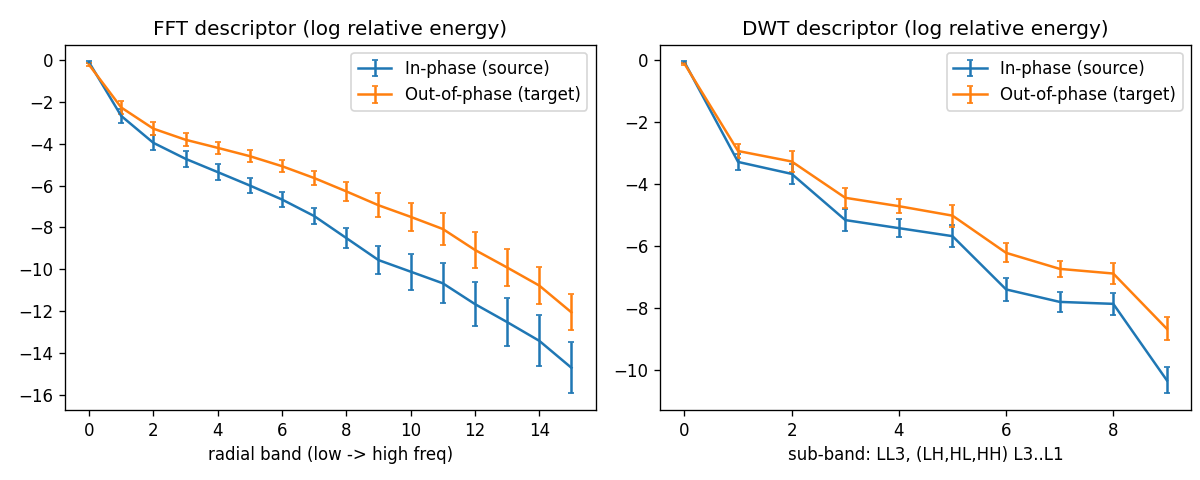
\includegraphics[width=\linewidth]{figures/freq_analysis_spectra.png}\\[-1mm]
    {\tiny Same anatomy, different MR sequence: OOP has more high-frequency energy (FFT bands, left; DWT sub-bands, right).}
  \end{columns}
\end{frame}

\begin{frame}{Dataset, task and objectives}
  \begin{columns}[T]
    \column{0.5\textwidth}
    \textbf{Dataset: CHAOS challenge} \cite{kavur2021chaos} (MR, T1-DUAL)
    \begin{itemize}\small
      \item 20 patients, 647 axial slices (26--50 per patient), $256\times256$ / $288\times288$, resized to $256^2$
      \item Labels: liver, right kidney, left kidney, spleen (+ background) = 5 classes
      \item \textbf{Source}: in-phase (IP), all 20 volumes, used for training
      \item \textbf{Target}: out-of-phase (OOP), the 20 volumes arrive as an \emph{online stream}, one patient = one batch (paper protocol, no train/test split on target)
    \end{itemize}
    \column{0.48\textwidth}
    \textbf{Task}: 2-D multi-class \textbf{segmentation}\\[2mm]
    \textbf{Objectives}
    \begin{enumerate}\small
      \item Reproduce ODES \cite{islam2025odes} on CHAOS IP$\rightarrow$OOP.
      \item Replace its BN-statistics image-pruning score with an interpretable \textbf{FFT / DWT frequency-domain} shift score (FreqODES).
      \item Compare at equal annotation budget ($K=10,50,100\%$ slices, $b=1\%$ pixels).
    \end{enumerate}
    \textbf{Metrics}: Dice (DSC), Jaccard (IoU) per organ and mean; adaptation time; paired Wilcoxon test over the 20 patients.
  \end{columns}
\end{frame}

% =============================== BASE PAPER ===============================
\section{Base paper}
\begin{frame}{Base paper}
  \begin{block}{ODES: Online Domain Adaptation with Expert Guidance for Medical Image Segmentation}
    M.\,S.~Islam, S.~Nag, A.~Dutta, S.\,M.~Ahmed, F.\,F.~Niloy, S.~Bera, A.\,K.~Roy-Chowdhury\\
    University of California, Riverside --- \textbf{MICCAI 2025} \cite{islam2025odes}. Code: \texttt{github.com/ShazidAraf/ODES}
  \end{block}
  \begin{itemize}
    \item First active-learning based \emph{online} UDA framework for medical segmentation: source-free, storage-free, one pass per batch.
    \item Four stages per incoming patient: \textbf{infer $\rightarrow$ prune images $\rightarrow$ acquire patch labels $\rightarrow$ update BN layers}.
    \item Contributions: (i) \textbf{image pruning} by BN-statistics KL divergence; (ii) \textbf{diversity-aware acquisition} (entropy $\times$ regional impurity $\times$ farthest-first diversity map).
    \item Evaluated on CHAOS IP$\rightarrow$OOP, CHAOS$\rightarrow$DUKE, BMC$\rightarrow$RUNMC; beats TENT, CoTTA, SaTTCA, \dots
  \end{itemize}
\end{frame}

\begin{frame}{ODES architecture}
  \centering
  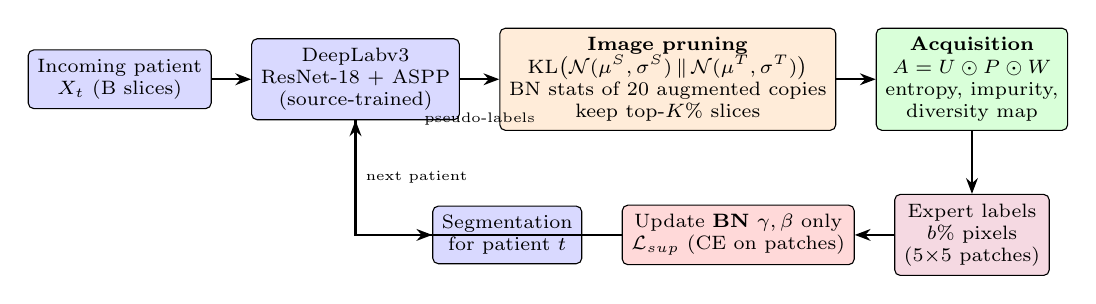
\begin{tikzpicture}[node distance=4mm and 5mm]
    \node[blk=blue] (in) {Incoming patient\\$X_t$ (B slices)};
    \node[blk=blue, right=of in] (net) {DeepLabv3\\ResNet-18 + ASPP\\(source-trained)};
    \node[blk=orange, right=of net] (prune) {\textbf{Image pruning}\\KL$\big(\mathcal{N}(\mu^S,\sigma^S)\,\|\,\mathcal{N}(\mu^{T},\sigma^{T})\big)$\\BN stats of 20 augmented copies\\keep top-$K\%$ slices};
    \node[blk=green, right=of prune] (acq) {\textbf{Acquisition}\\$A=U\odot P\odot W$\\entropy, impurity,\\diversity map};
    \node[blk=purple, below=8mm of acq] (exp) {Expert labels\\$b\%$ pixels\\(5$\times$5 patches)};
    \node[blk=red, left=of exp] (upd) {Update \textbf{BN} $\gamma,\beta$ only\\$\mathcal{L}_{sup}$ (CE on patches)};
    \node[blk=blue, left=of upd] (out) {Segmentation\\for patient $t$};
    \draw[arr] (in) -- (net); \draw[arr] (net) -- node[below=3mm,font=\tiny]{pseudo-labels} (prune);
    \draw[arr] (prune) -- (acq); \draw[arr] (acq) -- (exp); \draw[arr] (exp) -- (upd);
    \draw[arr] (upd) -| node[pos=0.75,right,font=\tiny]{next patient} (net);
    \draw[arr] (net) |- (out);
  \end{tikzpicture}
  \vspace{2mm}
  \begin{itemize}\small
    \item \textbf{Backbone}: DeepLabv3 \cite{chen2017deeplab}, ResNet-18 encoder (ImageNet init), ASPP, low-level skip, 5-class head.
    \item \textbf{Pruning}: each slice is augmented (flip / rotation), passed through a copy of the net; BN statistics of the last 9 BN layers are compared with source running statistics (Eq.\,1 of \cite{islam2025odes}).
    \item \textbf{Acquisition}: $U$ = patch-mean entropy, $P$ = regional impurity \cite{xie2022ripu}, $W$ = Gaussian map around farthest-first-traversal picks (spatial $\times$ feature).
  \end{itemize}
\end{frame}

\begin{frame}{Replicated vs.\ reported results (CHAOS IP $\rightarrow$ OOP, $b=1\%$)}
  \begin{table}
  \centering\scriptsize
  \caption{Dice (\%) per organ; Jaccard (IoU, \%) mean. Paper values from Table~1 of \cite{islam2025odes}.}
  \begin{tabular}{llcccccc}
    \toprule
    & Setting & Liver & L.\,Kidney & R.\,Kidney & Spleen & \textbf{Mean DSC} & \textbf{Mean IoU} \\
    \midrule
    \multirow{2}{*}{Source only} & Paper & 87.77 & 37.97 & 18.92 & 67.31 & 52.99 & -- \\
     & Ours & \DsourceonlyLiver & \DsourceonlyLK & \DsourceonlyRK & \DsourceonlySpleen & \Dsourceonly & \Jsourceonly \\
    \midrule
    \multirow{2}{*}{ODES $K{=}100$} & Paper & 88.90 & 72.41 & 74.55 & 78.56 & 78.61 & -- \\
     & Ours & \DODESKLiver & \DODESKLK & \DODESKRK & \DODESKSpleen & \textbf{\DODESK} & \JODESK \\
    \midrule
    \multirow{2}{*}{ODES $K{=}50$} & Paper & 89.13 & 72.30 & 74.43 & 78.36 & 78.56 & -- \\
     & Ours & \DBNKFiftyLiver & \DBNKFiftyLK & \DBNKFiftyRK & \DBNKFiftySpleen & \textbf{\DBNKFifty} & \JBNKFifty \\
    \midrule
    \multirow{2}{*}{ODES $K{=}10$} & Paper & 88.41 & 71.45 & 70.22 & 77.12 & 76.80 & -- \\
     & Ours & \DBNKTenLiver & \DBNKTenLK & \DBNKTenRK & \DBNKTenSpleen & \textbf{\DBNKTen} & \JBNKTen \\
    \bottomrule
  \end{tabular}
  \end{table}
  \small
  \begin{itemize}
    \item Source-only and adapted results are within $\approx$2 DSC of the paper; the adaptation gain (\Dsourceonly$\rightarrow$\DODESK, $\approx+25$) and the $K$ trend (100 $\approx$ 50 $>$ 10) are reproduced.
    \item No source checkpoint or training recipe is released, so we trained our own source model; organ-level differences (e.g.\ kidneys) come from that.
    \item Paper reports no Jaccard; ours is measured per volume.
  \end{itemize}
\end{frame}

\begin{frame}{Qualitative results: input, ground truth, predicted masks}
  \centering
  \IfFileExists{figures/qualitative.png}{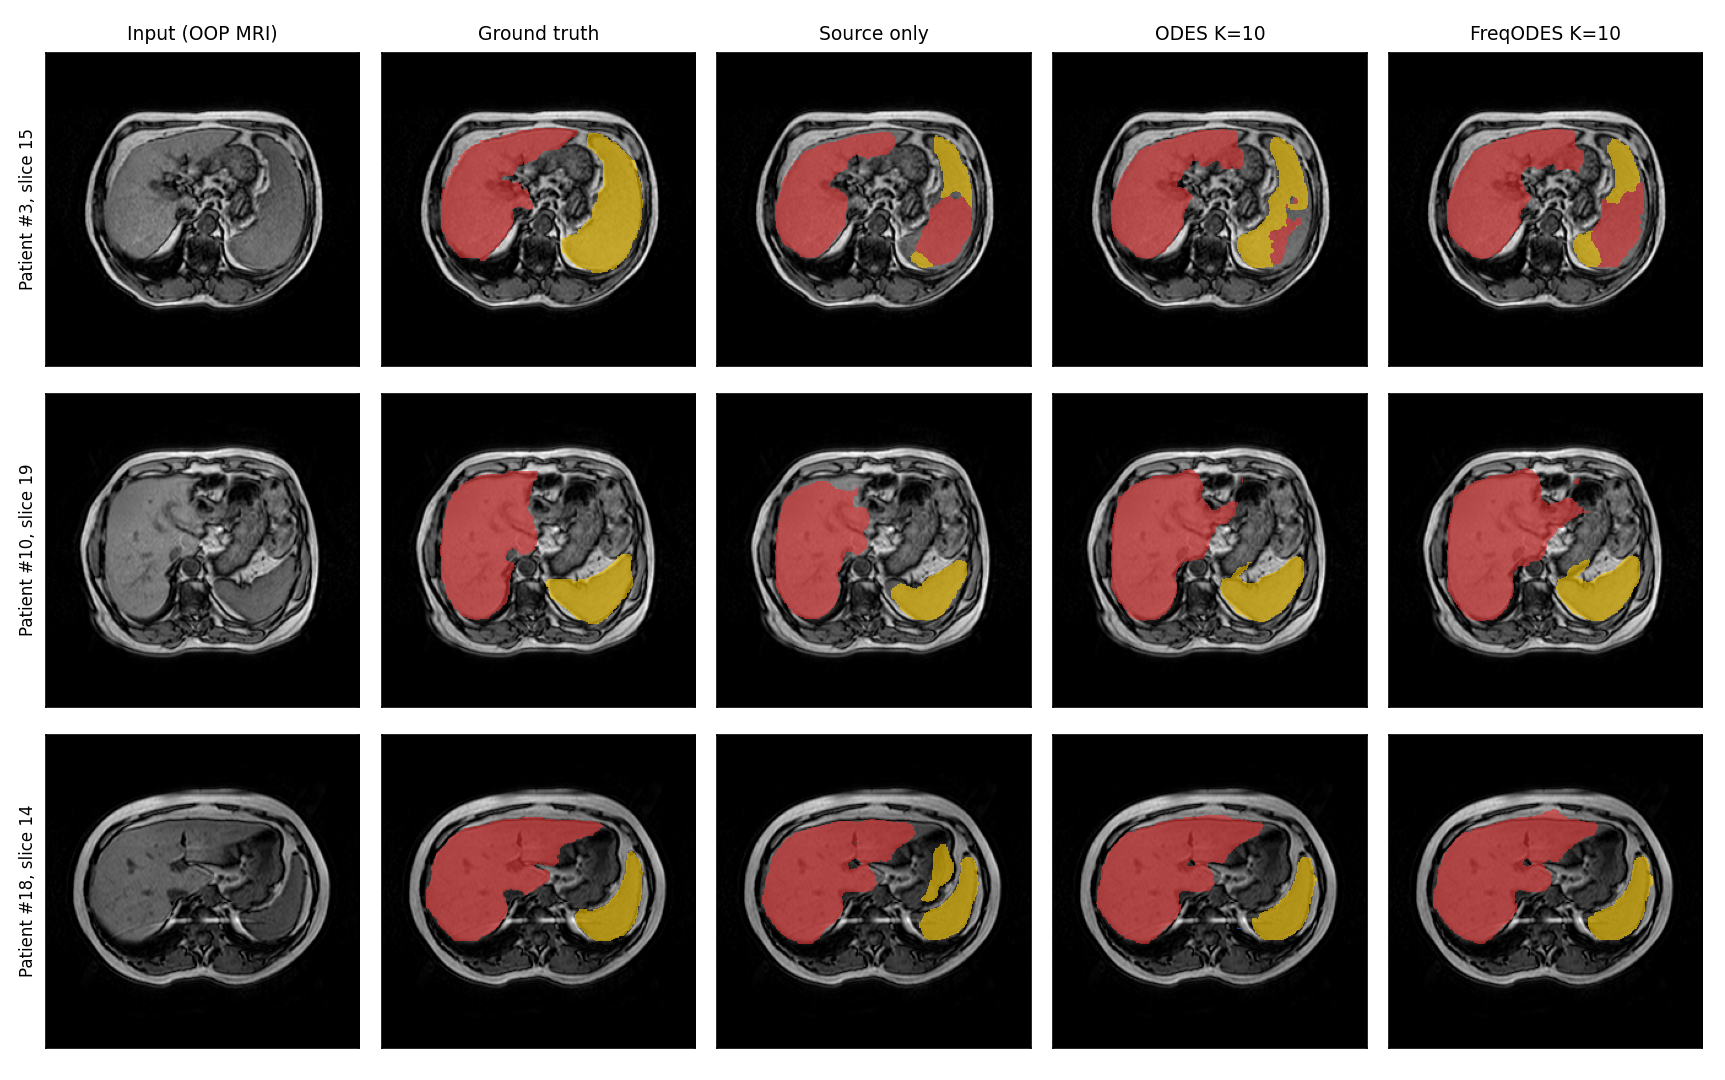
\includegraphics[height=0.78\textheight]{figures/qualitative.png}}{\fbox{\parbox{0.6\linewidth}{\centering qualitative.png is produced by \texttt{make\_report.py} from the saved predictions}}}\\
  {\scriptsize Red: liver, green: right kidney, blue: left kidney, yellow: spleen. Three target (OOP) patients, slice with largest organ area.}
\end{frame}

% =============================== IMPLEMENTATION ===============================
\section{Implementation}
\begin{frame}[fragile]{Code structure and training settings}
  \begin{columns}[T]
    \column{0.5\textwidth}
    \scriptsize
\begin{verbatim}
prepare_chaos.py   DICOM/PNG -> (D,H,W) tif stacks
dataloader/        Stack_Loader: one patient = batch
model/             DeepLabv3 (ResNet-18 + ASPP)
train_source.py    source training (CE + Dice)
methods/ODES.py    pruning, acquisition, BN update
methods/freq_shift.py  NEW: FFT / DWT shift score
FFT_weight_2.py    diversity map (missing upstream,
                   re-implemented from the paper)
demo_ODES.py       online loop + Dice / IoU eval
run_all.sh         21-run experiment sweep
make_report.py     tables, plots, LaTeX numbers
\end{verbatim}
    \normalsize\small
    Upstream repo had no training script, no checkpoint and a missing module; we added these and fixed CPU/GPU and a stale-variable bug.
    \column{0.48\textwidth}
    \begin{table}\scriptsize\centering
    \caption{Training / adaptation settings}
    \begin{tabular}{ll}
      \toprule
      Framework & PyTorch 2, timm \\
      Source optimiser & Adam, lr $10^{-3}$, wd $10^{-4}$, cosine \\
      Batch size / epochs & 8 / 25 \\
      Loss & CE + Dice \\
      Augmentation & flips, $90^\circ$ rot., intensity jitter \\
      Adaptation optimiser & Adam, lr $10^{-2}$, 1 step / patient \\
      Updated params & BN $\gamma,\beta$ only \\
      Budget & $b=1\%$ px, $K\in\{10,50,100\}\%$ \\
      Hardware & NVIDIA Tesla T4 (Colab) \\
      Seed & 1337 (all runs) \\
      \bottomrule
    \end{tabular}
    \end{table}
  \end{columns}
\end{frame}

\begin{frame}{Training log and curves}
  \begin{columns}[T]
    \column{0.48\textwidth}
    \centering
    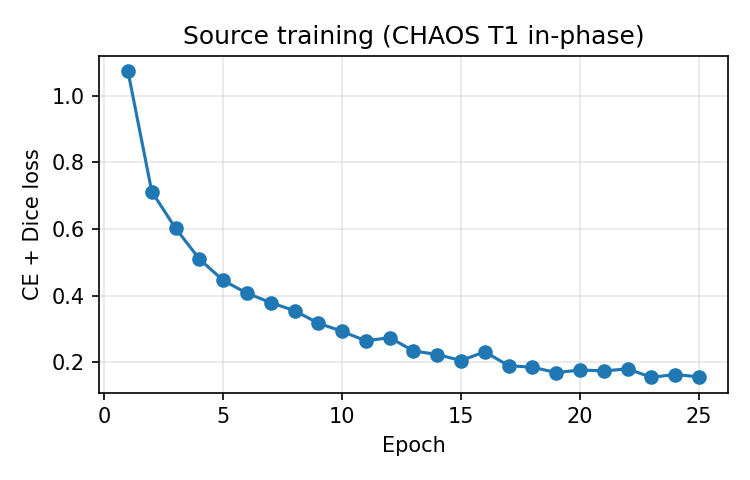
\includegraphics[width=\linewidth]{figures/train_loss.png}\\
    {\scriptsize Source training loss (25 epochs, 647 IP slices): $1.07\rightarrow0.16$.}
    \column{0.50\textwidth}
    \centering
    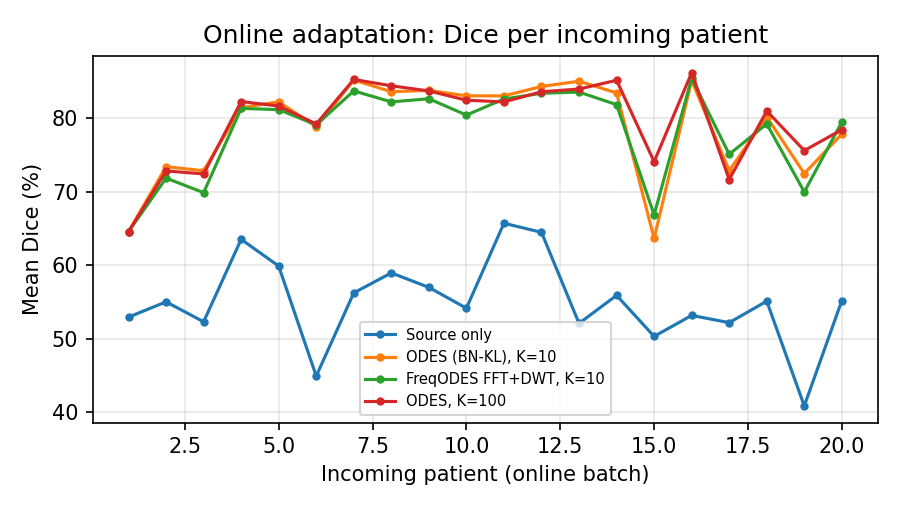
\includegraphics[width=\linewidth]{figures/online_dice.png}\\
    {\scriptsize Online adaptation: mean Dice of each incoming target patient. Expert-guided BN updates lift every patient above source-only.}
  \end{columns}
\end{frame}

% =============================== MODIFICATION ===============================
\section{Modification: FreqODES}
\begin{frame}{What we changed: frequency-domain image pruning}
  \begin{columns}[T]
    \column{0.52\textwidth}
    \small
    \textbf{Hypothesis}: MR sequence / scanner shift is directly visible as a change in spatial-frequency energy, so it can be detected from the image itself, without the network.
    \begin{itemize}\small
      \item \textbf{FFT descriptor}: log fraction of energy in 16 concentric radial bands of $|\mathcal{F}(x)|^2$.
      \item \textbf{DWT descriptor}: log relative energy of LL$_3$ and LH/HL/HH sub-bands of a 3-level Haar DWT.
      \item Reference $\mu_f,\sigma_f$ from 200 random source slices.
      \item Shift score $D_{freq}(x)=\frac{1}{d}\sum_f\big(\frac{\phi_f(x)-\mu_f}{\sigma_f}\big)^2$
      \item \textbf{Fused}: $D=\lambda\hat D_{BN}+(1-\lambda)\hat D_{freq}$
    \end{itemize}
    Only Stage 3 changes; backbone, acquisition, update and budgets are identical $\Rightarrow$ fair comparison.
    \column{0.46\textwidth}
    \centering
    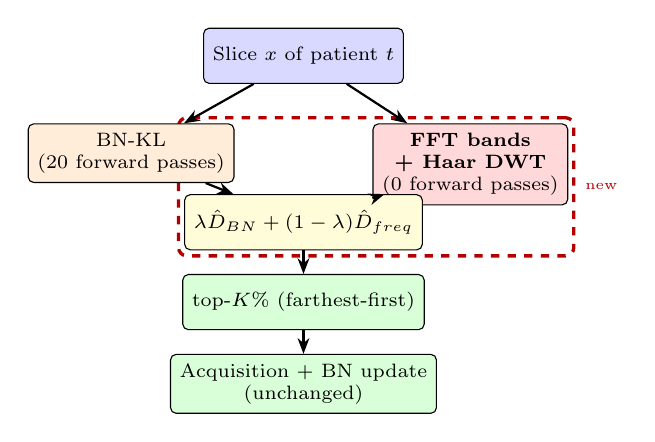
\begin{tikzpicture}[node distance=3mm]
      \node[blk=blue] (x) {Slice $x$ of patient $t$};
      \node[blk=orange, below left=5mm and -4mm of x] (bn) {BN-KL\\(20 forward passes)};
      \node[blk=red, below right=5mm and -4mm of x] (fq) {\textbf{FFT bands}\\\textbf{+ Haar DWT}\\(0 forward passes)};
      \node[blk=yellow, below=14mm of x] (fuse) {$\lambda\hat D_{BN}+(1-\lambda)\hat D_{freq}$};
      \node[blk=green, below=3mm of fuse] (sel) {top-$K\%$ (farthest-first)};
      \node[blk=green, below=3mm of sel] (rest) {Acquisition + BN update\\(unchanged)};
      \draw[arr] (x) -- (bn); \draw[arr] (x) -- (fq);
      \draw[arr] (bn) -- (fuse); \draw[arr] (fq) -- (fuse);
      \draw[arr] (fuse) -- (sel); \draw[arr] (sel) -- (rest);
      \begin{scope}[on background layer]
        \node[new, fit=(fq)(fuse), inner sep=2pt, label={[font=\tiny,red!70!black]right:new}] {};
      \end{scope}
    \end{tikzpicture}
  \end{columns}
\end{frame}

\begin{frame}{Does the frequency score detect the shift?}
  \centering
  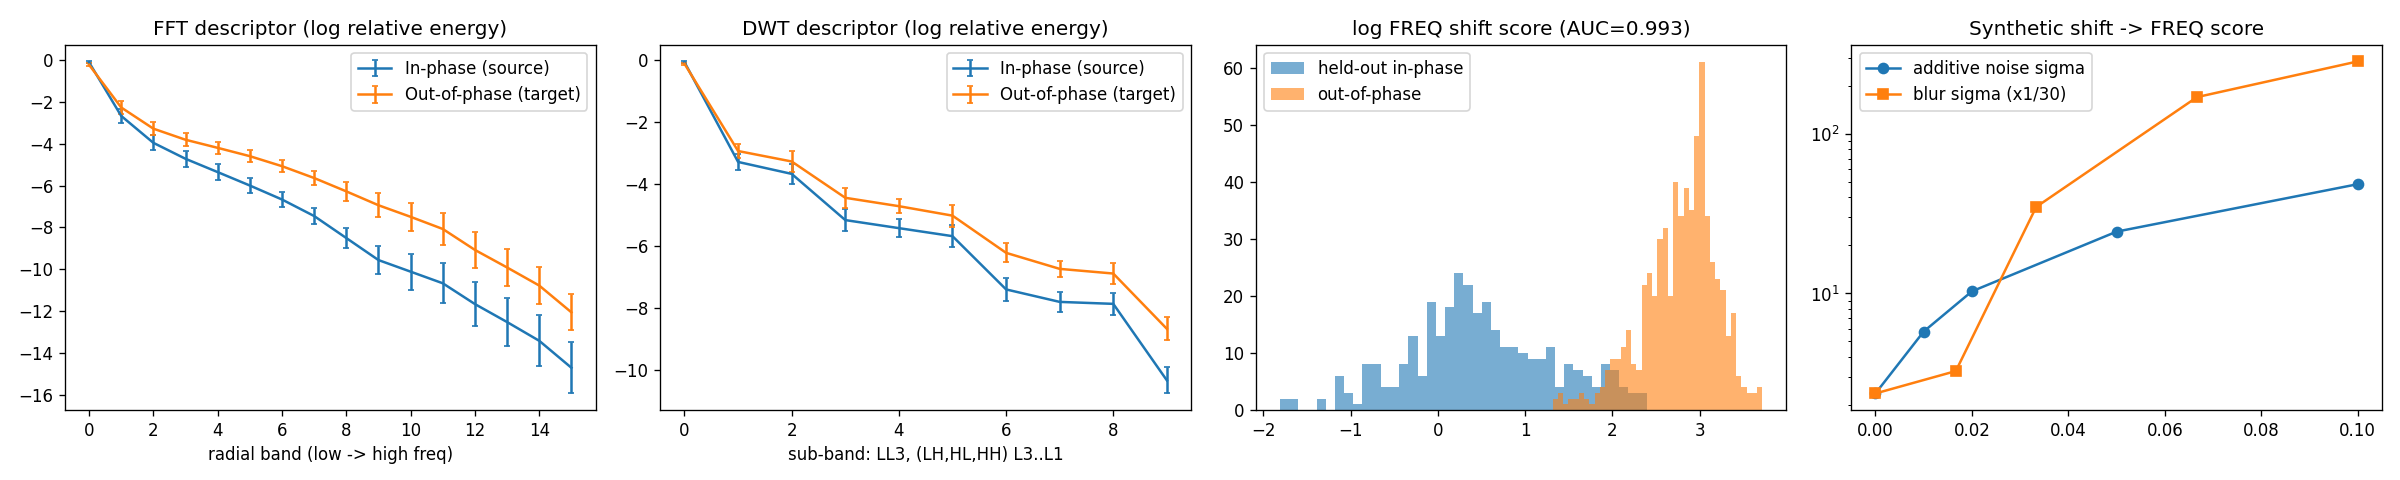
\includegraphics[width=\linewidth]{figures/freq_analysis.png}
  \begin{table}\scriptsize\centering
  \caption{Separating held-out IP slices (10 patients) from OOP slices with the shift score alone.}
  \begin{tabular}{lccc}
    \toprule
    Descriptor & FFT & DWT & FFT+DWT \\
    ROC-AUC & \textbf{\AUCFFT} & \AUCDWT & \AUCFREQ \\
    \bottomrule
  \end{tabular}
  \end{table}
  \vspace{-2mm}
  {\scriptsize OOP slices carry systematically more high-frequency energy; the score also grows monotonically with synthetic noise and blur.}
\end{frame}

\begin{frame}{FreqODES v1 (frequency score alone) vs.\ ODES, single seed}
  \begin{table}\scriptsize\centering
  \caption{Same data, model, seed and budget ($b=1\%$). DSC / IoU in \%, time = full online pass over 20 patients on a T4. $p$: paired Wilcoxon vs.\ ODES at the same $K$.}
  \begin{tabular}{lcccc@{\hskip 6mm}cccc}
    \toprule
    & \multicolumn{4}{c}{$K=10\%$ of slices} & \multicolumn{4}{c}{$K=50\%$ of slices} \\
    Pruning score & DSC & IoU & $p$ & Time (s) & DSC & IoU & $p$ & Time (s) \\
    \midrule
    BN-KL (ODES, replicated) & \textbf{\DBNKTen} & \JBNKTen & -- & \TBNKTen & \DBNKFifty & \JBNKFifty & -- & \TBNKFifty \\
    FFT (FreqODES) & \DFFTKTen & \JFFTKTen & \PFFTKTen & \TFFTKTen & \DFFTKFifty & \JFFTKFifty & \PFFTKFifty & \TFFTKFifty \\
    DWT (FreqODES) & \DDWTKTen & \JDWTKTen & \PDWTKTen & \TDWTKTen & \DDWTKFifty & \JDWTKFifty & \PDWTKFifty & \TDWTKFifty \\
    FFT+DWT (FreqODES) & \DFREQKTen & \JFREQKTen & \PFREQKTen & \TFREQKTen & \DFREQKFifty & \JFREQKFifty & \PFREQKFifty & \TFREQKFifty \\
    Fused, $\lambda{=}0.5$ & \DFUSEDKTenLFifty & \JFUSEDKTenLFifty & \PFUSEDKTenLFifty & \TFUSEDKTenLFifty & \textbf{\DFUSEDKFiftyLFifty} & \JFUSEDKFiftyLFifty & \PFUSEDKFiftyLFifty & \TFUSEDKFiftyLFifty \\
    Random & \DRANDOMKTen & \JRANDOMKTen & \PRANDOMKTen & \TRANDOMKTen & \DRANDOMKFifty & \JRANDOMKFifty & \PRANDOMKFifty & \TRANDOMKFifty \\
    \midrule
    \multicolumn{9}{l}{All slices ($K=100$): DSC \DODESK, IoU \JODESK \quad Source only: DSC \Dsourceonly, IoU \Jsourceonly} \\
    \bottomrule
  \end{tabular}
  \end{table}
  \centering
  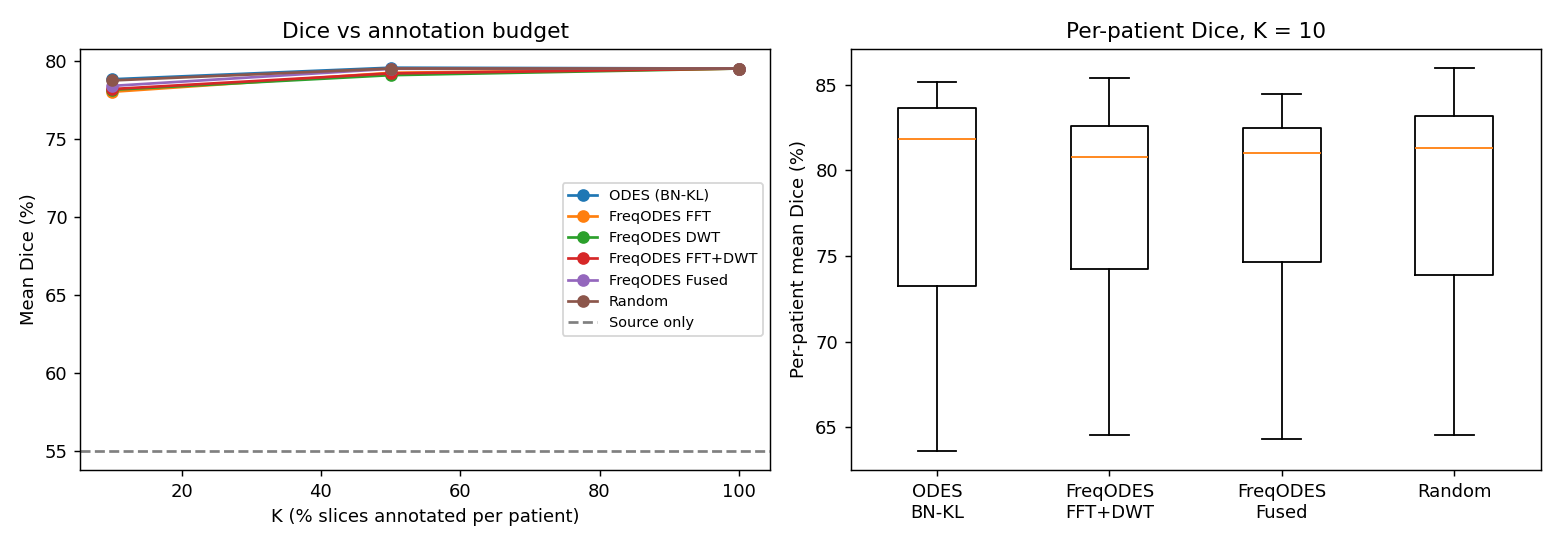
\includegraphics[height=0.3\textheight]{figures/dice_vs_budget.png}
\end{frame}

\begin{frame}{Ablations: pruning $\times$ diversity weighting, and fusion weight}
  \begin{columns}[T]
    \column{0.48\textwidth}
    \begin{table}\scriptsize\centering
    \caption{Mean DSC at $K=10$ (cf.\ Table 3 of \cite{islam2025odes}).}
    \begin{tabular}{lcc}
      \toprule
      Image pruning & D.W.\ off & D.W.\ on \\
      \midrule
      BN-KL (ODES) & \DBNKTennoDW & \DBNKTen \\
      FFT+DWT (ours) & \DFREQKTennoDW & \DFREQKTen \\
      Random & \DRANDOMKTennoDW & \DRANDOMKTen \\
      \midrule
      Paper (BN / random) & 75.88 / 74.32 & 76.80 / 75.41 \\
      \bottomrule
    \end{tabular}
    \end{table}
    \column{0.48\textwidth}
    \begin{table}\scriptsize\centering
    \caption{Fusion weight $\lambda$ ($K=10$).}
    \begin{tabular}{lc}
      \toprule
      $\lambda$ & Mean DSC \\
      \midrule
      0 (pure frequency) & \DFREQKTen \\
      0.25 & \DFUSEDKTenLQuarter \\
      0.5 & \DFUSEDKTenLFifty \\
      0.75 & \DFUSEDKTenLThreeQ \\
      1 (pure BN = ODES) & \DBNKTen \\
      \bottomrule
    \end{tabular}
    \end{table}
  \end{columns}
  \small
  Mixing a little BN information into the frequency score ($\lambda=0.25$) gives the best $K=10$ result (\DFUSEDKTenLQuarter\ vs.\ \DBNKTen, not significant, $p=0.75$); diversity weighting changes DSC by $\le 0.2$ in our runs, much less than reported in the paper.
\end{frame}

\begin{frame}{Analysis: why v1 alone did not beat ODES (and what it led to)}
  \begin{itemize}\small
    \item \textbf{Where it helps}: best shift \emph{detector} (AUC \AUCFFT), interpretable, needs no forward passes $\Rightarrow$ full online pass \TFREQKTen\,s vs.\ \TBNKTen\,s ($\approx 35\%$ faster). The fused score matches ODES at both budgets (\DFUSEDKFiftyLFifty\ vs.\ \DBNKFifty\ at $K=50$, $p=\PFUSEDKFiftyLFifty$) and with $\lambda=0.25$ reaches \DFUSEDKTenLQuarter\ at $K=10$.
    \item \textbf{Where it hurts}: pure frequency scores trail ODES by 0.6--0.8 DSC at $K=10$ (FFT: \DiffFFTKTen, $p=\PFFTKTen$) and by 0.3--0.5 at $K=50$.
    \item \textbf{Mismatch between objective and score}: the most frequency-shifted slices are the volume extremes (few or tiny organs, mostly background); labelling them teaches the BN layers little. BN-KL measures what \emph{the network} finds unusual, which correlates better with segmentation error.
    \item \textbf{Small, homogeneous shift}: IP$\rightarrow$OOP shift is global, so nearly every OOP slice is ``shifted''; ranking among them is what matters, and random pruning is already strong (\DRANDOMKTen, $p=\PRANDOMKTen$).
    \item \textbf{Fix}: a slice is worth labelling if it is \emph{shifted} \textbf{and} the model is \emph{unsure} about it $\Rightarrow$ multiply the frequency score by model uncertainty (next slide), and evaluate over 3 seeds.
  \end{itemize}
\end{frame}

\begin{frame}{FreqODES-U: frequency shift $\times$ model uncertainty}
  \begin{columns}[T]
    \column{0.52\textwidth}
    \small
    \textbf{Slice score}
    \[
      S(x_j)=\underbrace{\hat D_{freq}(x_j)}_{\text{FFT+DWT shift}}\;\times\;\underbrace{\hat H(x_j)}_{\text{mean pixel entropy}}
    \]
    \begin{itemize}\scriptsize
      \item $\hat D_{freq}$: v1 frequency score; $\hat H$: mean entropy of the softmax prediction of the slice; each normalised by its batch maximum.
      \item $\hat H$ reuses the inference prediction ODES already makes $\Rightarrow$ still \textbf{0 extra forward passes}.
      \item Pre-registered design (v2): $\hat D_{freq}\times$ organ area $\times\hat H$, with two ablations (drop one factor each). The ablation $\hat D_{freq}\times\hat H$ was best; we report \emph{all} variants.
      \item Protocol: 3 seeds (1, 2, 12345) $\times$ 20 patients; paired Wilcoxon over the 60 patient-runs.
    \end{itemize}
    \column{0.46\textwidth}
    \centering
    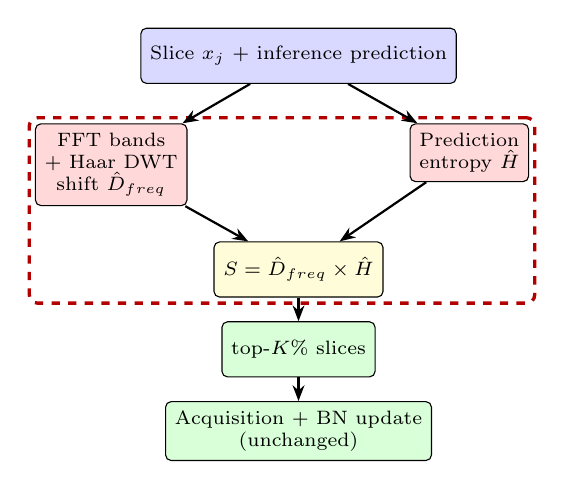
\begin{tikzpicture}[node distance=3mm]
      \node[blk=blue] (x) {Slice $x_j$ + inference prediction};
      \node[blk=red, below left=5mm and -6mm of x] (fq) {FFT bands\\+ Haar DWT\\shift $\hat D_{freq}$};
      \node[blk=red, below right=5mm and -6mm of x] (h) {Prediction\\entropy $\hat H$};
      \node[blk=yellow, below=20mm of x] (m) {$S=\hat D_{freq}\times\hat H$};
      \node[blk=green, below=3mm of m] (sel) {top-$K\%$ slices};
      \node[blk=green, below=3mm of sel] (rest) {Acquisition + BN update\\(unchanged)};
      \draw[arr] (x) -- (fq); \draw[arr] (x) -- (h);
      \draw[arr] (fq) -- (m); \draw[arr] (h) -- (m);
      \draw[arr] (m) -- (sel); \draw[arr] (sel) -- (rest);
      \begin{scope}[on background layer]
        \node[new, fit=(fq)(h)(m), inner sep=2pt] {};
      \end{scope}
    \end{tikzpicture}
  \end{columns}
\end{frame}

\begin{frame}{FreqODES-U results: 3 seeds, same model and budget}
  \begin{table}\scriptsize\centering
  \caption{Mean Dice (\%) $\pm$ std over 3 seeds; $\Delta$ and $p$: paired Wilcoxon vs.\ ODES over 60 patient-runs; time: full online pass (T4).}
  \begin{tabular}{lcccc@{\hskip 5mm}ccc}
    \toprule
    & \multicolumn{4}{c}{$K=10\%$ of slices} & \multicolumn{3}{c}{$K=50\%$ of slices} \\
    Selection score & DSC & $\Delta$ / $p$ & IoU & Time & DSC & $\Delta$ / $p$ & IoU \\
    \midrule
    ODES (BN-KL) & \VBnTenMean$\pm$\VBnTenStd & -- & \VBnTenIoU & \VBnTenTime\,s & \textbf{\VBnFiftyMean}$\pm$\VBnFiftyStd & -- & \VBnFiftyIoU \\
    v1: frequency & \VFqTenMean$\pm$\VFqTenStd & \VFqTenDiff\ / \VFqTenP & \VFqTenIoU & \VFqTenTime\,s & \VFqFiftyMean$\pm$\VFqFiftyStd & \VFqFiftyDiff\ / \VFqFiftyP & \VFqFiftyIoU \\
    v2: freq $\times$ area $\times$ unc. & \VFvTenMean$\pm$\VFvTenStd & \VFvTenDiff\ / \VFvTenP & \VFvTenIoU & \VFvTenTime\,s & \VFvFiftyMean$\pm$\VFvFiftyStd & \VFvFiftyDiff\ / \VFvFiftyP & \VFvFiftyIoU \\
    Ablation: freq $\times$ area & \VFaTenMean$\pm$\VFaTenStd & \VFaTenDiff\ / \VFaTenP & \VFaTenIoU & \VFaTenTime\,s & -- & -- & -- \\
    \textbf{FreqODES-U: freq $\times$ unc.} & \textbf{\VFeTenMean}$\pm$\VFeTenStd & \textbf{\VFeTenDiff\ / \VFeTenP} & \textbf{\VFeTenIoU} & \VFeTenTime\,s & \VFeFiftyMean$\pm$\VFeFiftyStd & \VFeFiftyDiff\ / \VFeFiftyP & \VFeFiftyIoU \\
    Random & \VRdTenMean$\pm$\VRdTenStd & \VRdTenDiff\ / \VRdTenP & \VRdTenIoU & \VRdTenTime\,s & \VRdFiftyMean$\pm$\VRdFiftyStd & \VRdFiftyDiff\ / \VRdFiftyP & \VRdFiftyIoU \\
    \bottomrule
  \end{tabular}
  \end{table}
  \vspace{-2mm}
  \centering
  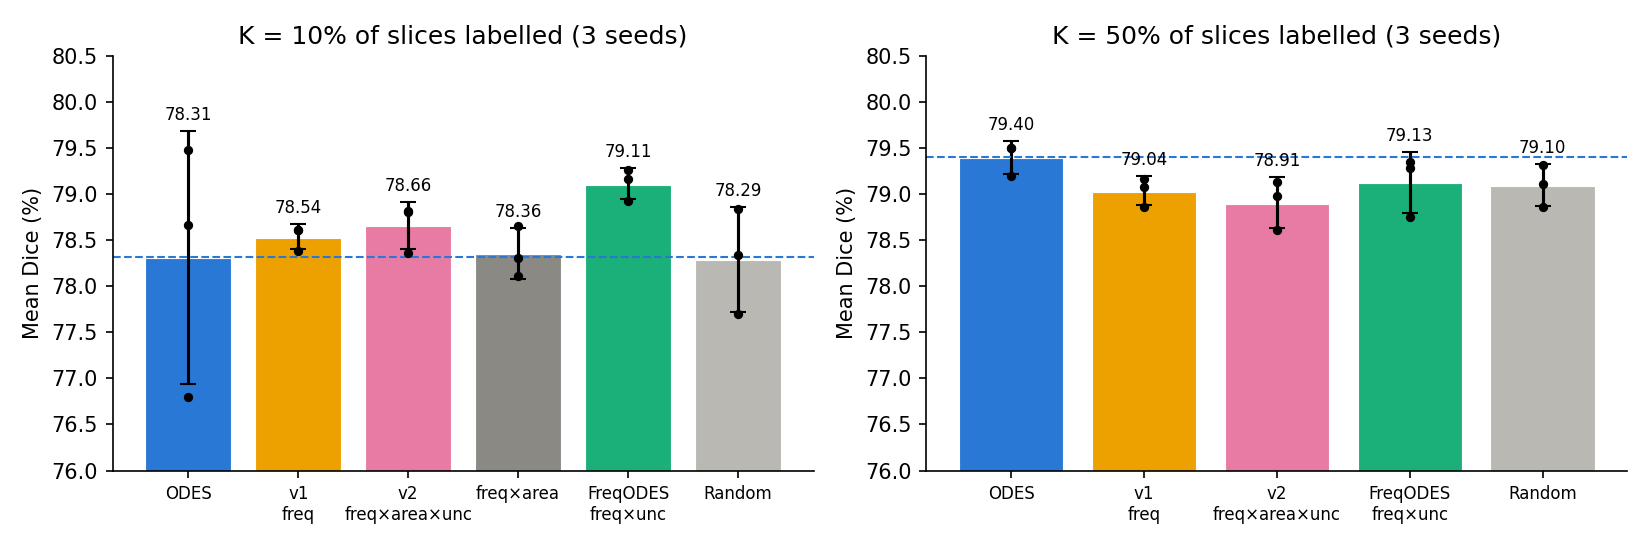
\includegraphics[height=0.27\textheight]{figures/v2_results.png}\\
  {\scriptsize At $K=10\%$ FreqODES-U beats ODES on every seed (\VFeTenSa, \VFeTenSb, \VFeTenSc\ vs.\ \VBnTenSa, \VBnTenSb, \VBnTenSc), 8$\times$ more stable, $\approx$33\% faster. At $K=50\%$ ODES stays best.}
\end{frame}

% =============================== CLOSING ===============================
\section{Conclusion}
\begin{frame}{Conclusion, contributions and references}
  \begin{columns}[T]
    \column{0.55\textwidth}
    \small
    \textbf{Conclusion}
    \begin{itemize}\scriptsize
      \item ODES reproduced on CHAOS IP$\rightarrow$OOP (\DODESK\ vs.\ 78.61 DSC at $K=100$) after completing the public code.
      \item v1: an interpretable FFT/DWT shift detector (AUC \AUCFFT), $\approx35\%$ cheaper, but alone it does not beat ODES: a good \emph{shift} detector is not automatically a good \emph{annotation-value} detector.
      \item \textbf{FreqODES-U} (frequency $\times$ uncertainty): \textbf{\VFeTenMean\ vs.\ \VBnTenMean\ DSC at $K=10\%$} ($\Delta$\VFeTenDiff, $p=\VFeTenP$, 3 seeds), more stable and $\approx$33\% faster; at $K=50\%$ ODES stays best (\VBnFiftyMean\ vs.\ \VFeFiftyMean).
      \item Caveats: best variant found in a pre-planned ablation; one dataset pair; 3 seeds. Next: CHAOS$\rightarrow$DUKE, more seeds.
    \end{itemize}
    \textbf{Member contributions}
    \begin{itemize}\scriptsize
      \item \MemberA: \textless contribution\textgreater
      \item \MemberB: \textless contribution\textgreater
    \end{itemize}
    \column{0.43\textwidth}
    \tiny
    \setbeamertemplate{bibliography item}[text]
    \begin{thebibliography}{9}
      \bibitem{islam2025odes} M.\,S.~Islam, S.~Nag, A.~Dutta, S.\,M.~Ahmed, F.\,F.~Niloy, S.~Bera, A.\,K.~Roy-Chowdhury. ODES: Online domain adaptation with expert guidance for medical image segmentation. \emph{MICCAI}, 2025.
      \bibitem{kavur2021chaos} A.\,E.~Kavur et al. CHAOS challenge -- combined (CT-MR) healthy abdominal organ segmentation. \emph{Medical Image Analysis} 69:101950, 2021.
      \bibitem{chen2017deeplab} L.-C.~Chen, G.~Papandreou, I.~Kokkinos, K.~Murphy, A.\,L.~Yuille. DeepLab: semantic image segmentation with deep convolutional nets, atrous convolution, and fully connected CRFs. \emph{IEEE TPAMI} 40(4):834--848, 2018.
      \bibitem{xie2022ripu} B.~Xie, L.~Yuan, S.~Li, C.\,H.~Liu, X.~Cheng. Towards fewer annotations: active learning via region impurity and prediction uncertainty for domain adaptive semantic segmentation. \emph{CVPR}, 2022.
    \end{thebibliography}
  \end{columns}
\end{frame}

\end{document}
